
\chapter{Architettura}                %crea il capitolo
%%%%%%%%%%%%%%%%%%%%%%%%%%%%%%%%%%%%%%%%%imposta l'intestazione di pagina
\lhead[\fancyplain{}{\bfseries\thepage}]{\fancyplain{}{\bfseries\rightmark}}
\pagenumbering{arabic}                  %mette i numeri arabi


L'applicazione \'e stata realizzata per la piattaforma mobile Android utilizzando il linguaggio di programmazione Kotlin, e altre librerie open-source. La parte client \'e stata scritta utilizzando il pattern MVP e utilizzando la classica organizzazione dei file di Android, differenziando quindi Activity, Fragment, Adapter e Servizi.\\
La parte server invece \'e stata realizzata utilizzando come BaaS Firebase e i suoi servizi offerti per la gestone del database, autenticazione, notifiche e storage.\\
Ogni servizio offerto da Firebase interagisce in maniera diretta o indiretta con tutti gli altri servizi,, che facilit\'a la gestisce dell'autenticazione, del database e dei uno storage online.\\

\newpage



\section{Server}                 %crea la sezione
La getione del backend \'e stata realizzata utilizzando la piattaforma Firebase e i suoi servizi.
I servizi utilizzati per la gestione del backend sono:
\begin{enumerate}
\item \textbf{Auth}: servizio per gestire l'autenticazione degli utenti
\item \textbf{Firestore}: database real-time per la memorizzazione di tutti i dati utilizzati dall'applicazione
\item \textbf{Storage}: spazio di archiviazione utilizzato per salvare gli avatar degli utenti e le immagini dei gruppi.
\item \textbf{Cloud Functions}: servizio utilizzato per monitorare i cambiamenti all'interno del database Firestore
\item \textbf{Cloud Messaging}: servizio utilizzato per gestire ed inviare notifiche ai dispositivi
\end{enumerate}


\begin{figure}[!hb]
  \centering
  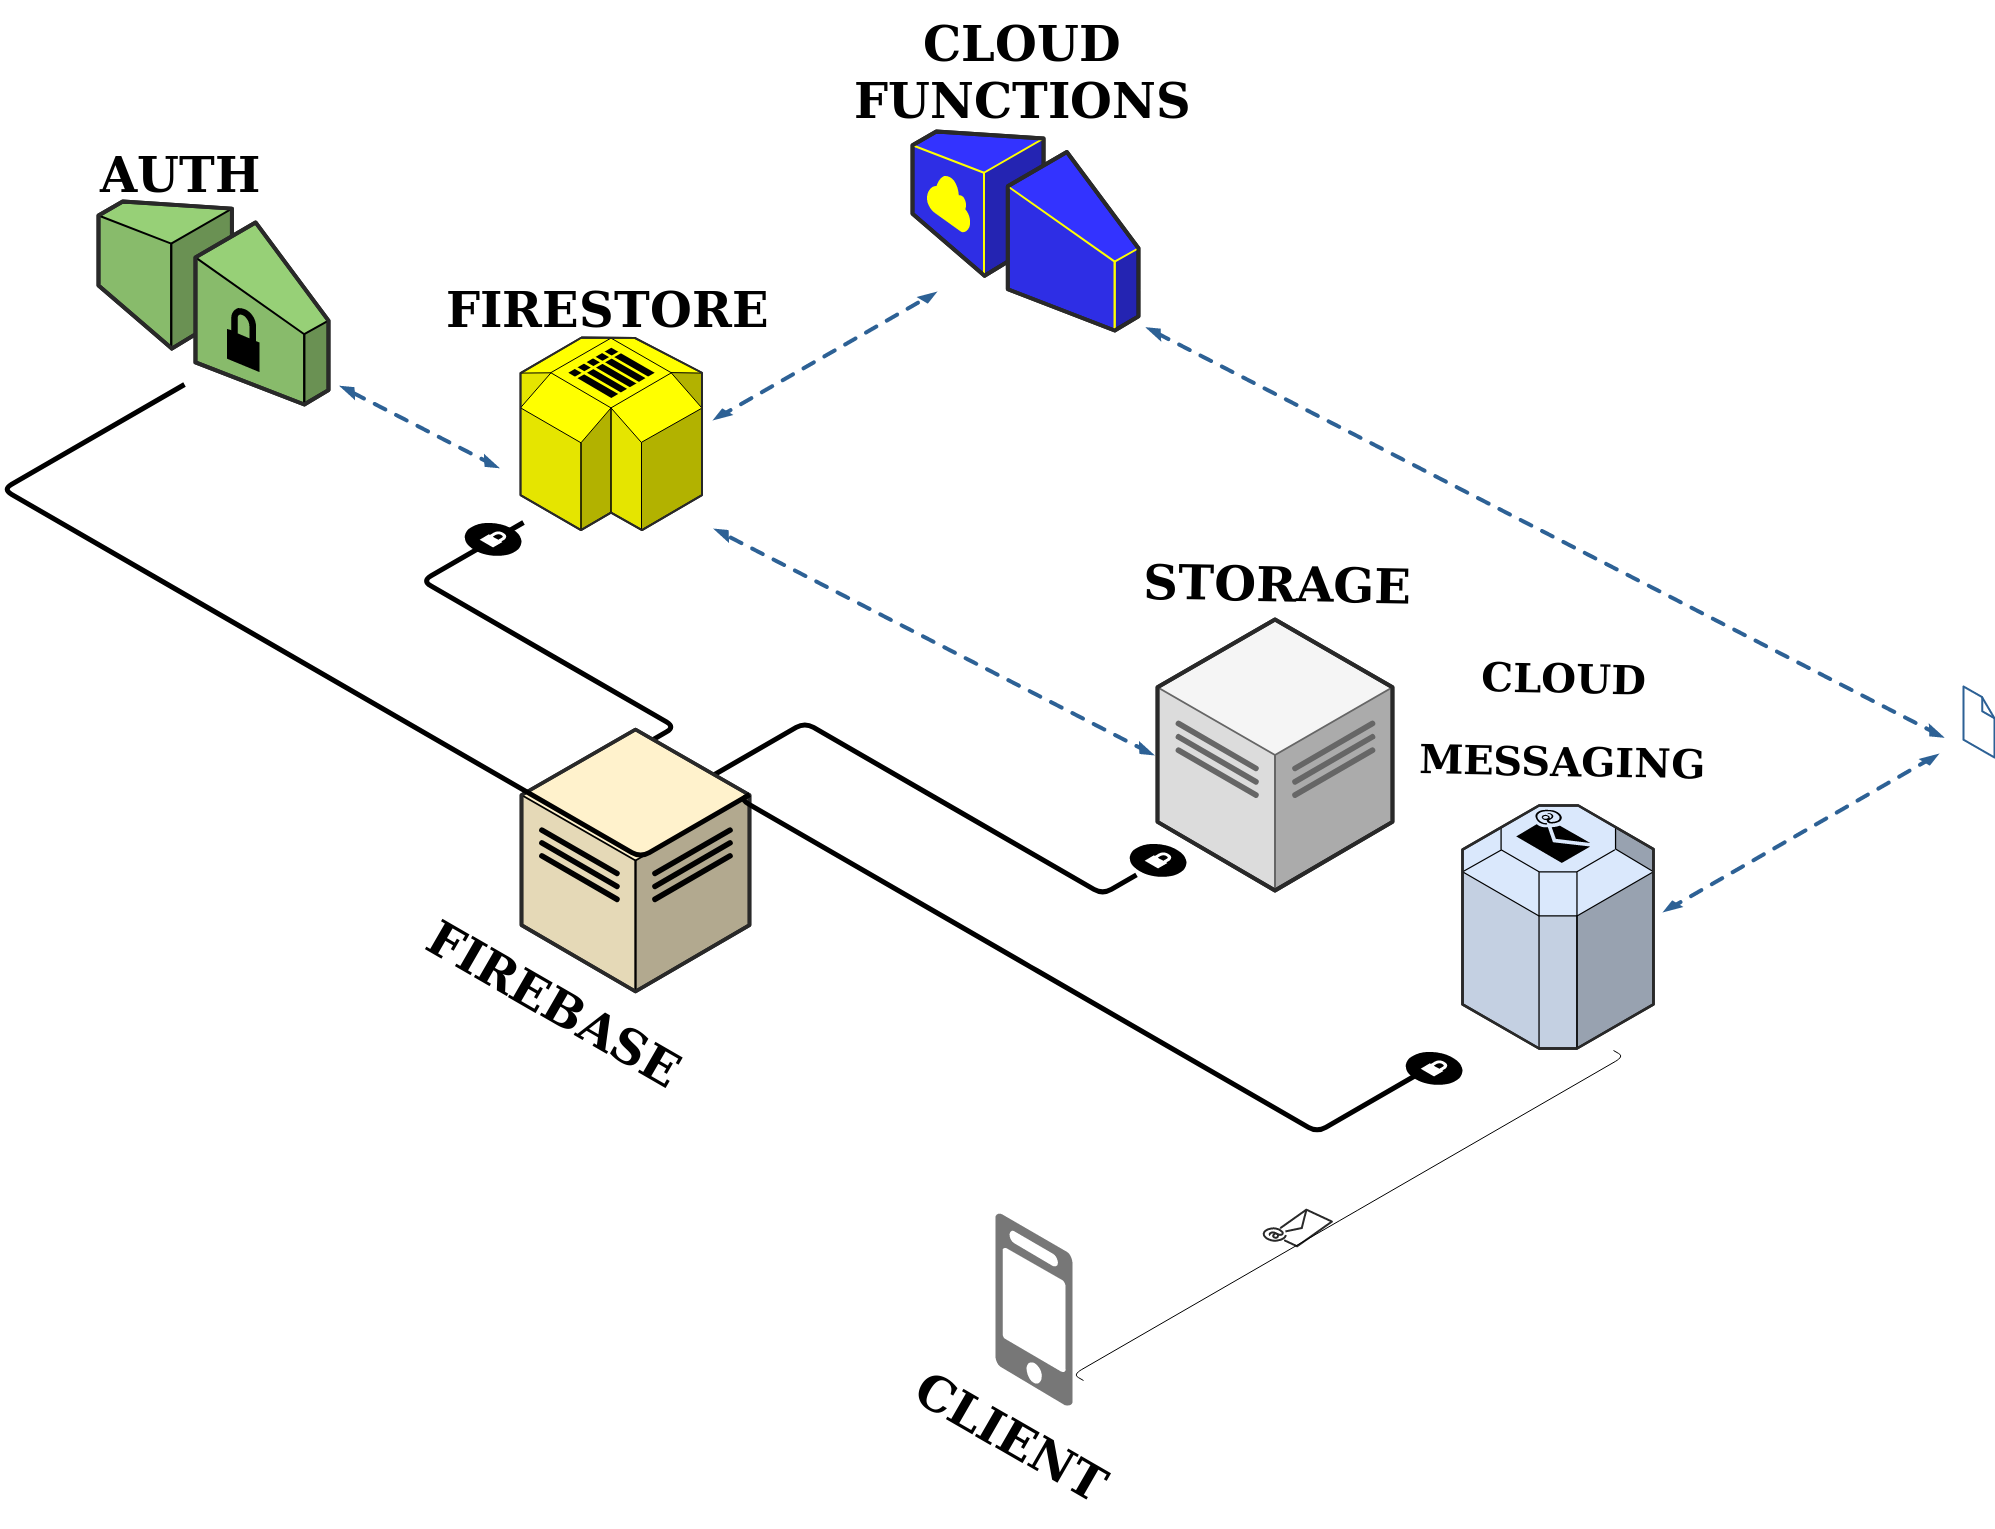
\includegraphics[width=0.8\textwidth]{immagini/server_arch.png}
  \caption{Server Architettura}\label{fig:Architettura Server}
\end{figure}

\subsection{Autenticazione}
I client connessi a Firebase, hanno la possibilit\'a di registrarsi attraverso email, e social login (Google,Faceook,Twitter). Una volta effettuata la registrazione, FirebaseAuth assegner\'a un identificativo univoco al nuovo client, memorizzando nei suoi server le informazioni basilari, quali: ID, nome, data di creazione, ultimo accesso, email, e provider (Email, Google, Faceook, Twitter).
\begin{figure}[!h]
  \centering
  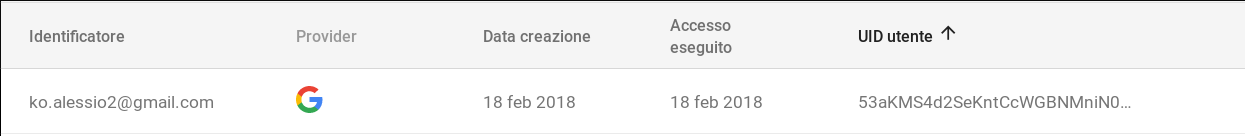
\includegraphics[width=1\textwidth]{immagini/firebase_auth_user.png}
  \caption{Firebase Auth User}\label{fig:Firebase User}
\end{figure}

Le informazioni salvate all'interno del servizio Firebase Auth sono differenti da quelle del database Firestore, di conseguenza per salvare ulteriori informazioni riguardanti l'utente, ogni volta che un client si registra su FirebaseAuth, verr\'a creato anche il suo rispettivo record all'interno del database Firestore.\\
Le informazioni aggiuntive salvate all'interno del database sono le seguenti:

\begin{itemize}
    \item \textbf{ID:}  identificativo univoco assegnato dal servizio FirebaseAuth
    \item \textbf{Name:} nome dell'utente, inserito in fase di registrazione
    \item \textbf{Email:} email univoca di registrazione dell'utente
    \item \textbf{PhotoUrl:} avatar opzionale dell'utente
    \item \textbf{GroupID:} gruppo di appartenenza univoco
    \item \textbf{TokenFCM:} stringa utilizzata per interagire con il servizio FCM
\end{itemize}

\newpage

\subsection{Storage}
Gli utenti hanno la possibilit\'a di salvare e personalizzare i propri avatar e gestire l'immagine del gruppo a cui appartengono, la memorizzazione di queste immagine viene fornita dal servizio Firebase Storage.
Il servizio offre la possibilit\'a di caricare online qualsiasi tipo di file sia attraverso l'SDK per i vari client sia attraverso il pannello di controllo di Firebase.\\
Ogni file presente sullo storage contiene il nome, la dimensione, il tipo e l'ultima modifica del file, oltre a queste informazioni sono presenti due link: il riferimento del file sullo storage e un URL pubblico che consente il download del file.

\begin{figure}[!hb]
  \centering
  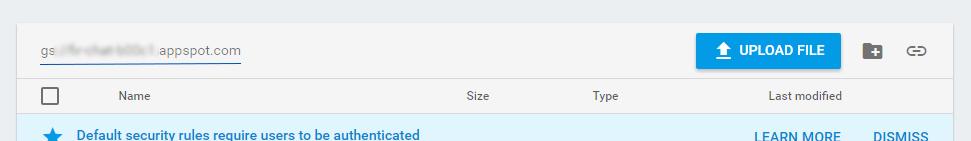
\includegraphics[width=1\textwidth]{immagini/firebase_storage.png}
  \caption{Firebase Storage}\label{fig:Firebase Storage}
\end{figure}

Il riferimento viene utilizzato dall'SDK per avere un identificativo del file all'interno dello storage, questo identificativo viene utilizzato dai client per scaricare il file applicando restrizioni di visibilit\'a, il link pubblico invece permette a chi lo possiede di visualizzare e scaricare il file(per motivi di sicurezza questo link pu\'o essere rigenerato).\\
L'organizzazione dei file presente all'interno dello storage \'e gerarhica, per separare le immagini degli utenti con le immagini dei gruppi, ogni immagine viene salvata nella rispettiva cartella, gli avatar vengono salvati nella cartella "UserAvatar" e come identificativo le immagini hanno l'ID dell'utente assegnato da Firestore, le immagini dei gruppi invece vengono salvate nella cartella "GroupAvatar" e utilizzano come identificativo l'ID del gruppo.
Assegnando un identificativo univoco ad ogni file \'e possibile fare riferimento a tutte le immagini sia attraverso il pannello di controllo di Firebase, sia utilizzando l'SDK.\\




\subsection{Notifiche}
Le notifiche vengono gestite dal server Cloud Messaging, che si occupa della memorizzazione, invio e ricezioni delle notifiche fra client e server.\\
La ricezione dei messaggi da parte di Cloud Messaging \'e possibile solo se si utilizza l'apposito SDK e si ottiene un token, necessario per inviare un messaggio ad un dispositivo specifico, il token di registrazione viene generato automaticamente dall'SDK all'avvio dell'applicazione.\\
L'SDK consente di visualizzare i messaggi ricevuti dal servizio e gestire la generazione e il cambiamento del token. Il token di registrazione pu\'o cambiare solo quando l'applicazione viene reinstallata, disinstallata o quando vengono eliminate le cache e i dati dal dispositivo.\\
I passi necessari per connette e ricevere i messaggi dal server FCM sono i seguenti:
\begin{itemize}
    \item Client attraverso una richiesta al server FCM, richiede un token
    \item Il server FCM, se la richiesta \'e valida, restituisce un token di registrazione
    \item Il client invia al database Firestore il token di registrazione
    \item Da questo momento il client utilizzando il token pu\'o inviare o ricevere messaggi connettendosi al server FCM con l'SDK o attraverso richieste HTTP/XMPP
\end{itemize}

\begin{figure}[!hb]
  \centering
  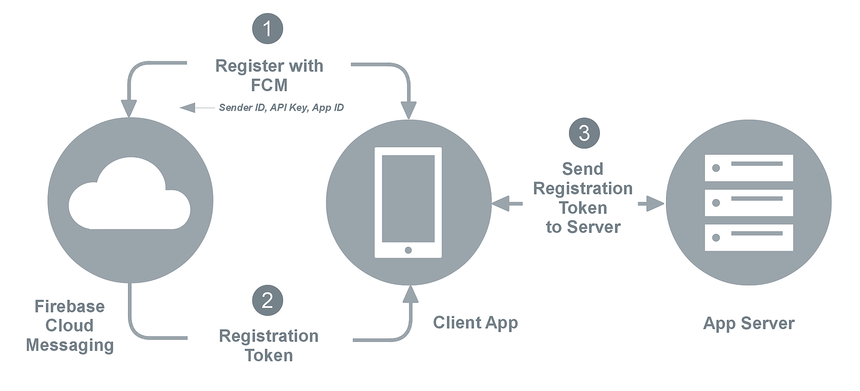
\includegraphics[width=0.65\textwidth]{immagini/fcm_token.png}
  \caption{Architettura Token FCM} \label{fig:Architettura Token FCM}
\end{figure}

\subsection{Database}
La tipologia di database utilizzato \'e ``Document Based'', Lorem ipsum dolor sit amet, consectetur adipisicing elit, sed do eiusmod tempor incididunt ut labore et dolore magna aliqua. Ut enim ad minim veniam, quis nostrud exercitation ullamco laboris nisi ut aliquip ex ea commodo consequat. Duis aute irure dolor in reprehenderit in voluptate velit esse cillum dolore eu fugiat nulla pariatur. Excepteur sint occaecat cupidatat non proident, sunt in culpa qui officia deserunt mollit anim id est laborum.\\
Il database \'e organizzato in due sole collezioni principali, la collezione degli utenti e la collezione dei gruppi.\\
La struttura di ogni utente \'e la segueda FCM nte:

\begin{table}[h]
\begin{center}
\begin{tabular}{|p{2cm}|p{2cm}|p{9cm}|}
    \hline
\textbf{Dato} & \textbf{Tipo}  & \textbf{Descrizione}\\ \hline
ID & Int & Identificativo univoco \\\hline
Name & String & nome dell'utente, inserito in fase di registrazione \\ \hline
Email & String &  email univoca di registrazione dell'utente \\ \hline
PhotoUrl & String & avatar opzionale dell'utente \\ \hline
GroupID & Int &  gruppo di appartenenza univoco \\ \hline
TokenFCM & String & stringa utilizzata per interagire con il servizio FCM \\
\hline
\end{tabular}
\caption[Dati Firestore]{Strutura collezione User}\label{tab:Strutture collezzione User}
\end{center}
\end{table}

L'identificativo ID assegnato all'utente \'e lo stesso dell'identificativo assegnato da Firebase Auth per avere una diretta associazione tra il servizio Firestore e Firebase Auth, il TokenFCM invece \'e generato dall'SDK del servizio Cloud Messaging.\\
Il nome, l'email, e l'avatar dell'utente vengono invece settati attraverso le informazioni recuperate quando si esegue la registrazione tramite social login, e tramite email.\\
Infine il groupID \'e assegnato al memomento della registrazione quando quando l'utente seleziona il gruppo di appartenenza oppure sceglie di crearne uno nuovo.




\begin{table}[h]
\begin{center}
\begin{tabular}{|l|l|p{10cm}|}
    \hline
\textbf{Dato} & \textbf{Tipo}  & \textbf{Descrizione}\\ \hline
ID & Int & Identificativo univoco \\\hline
Name & String & Nome del gruppo \\ \hline
Date & Date & Data di creazione del gruppo \\ \hline
TokenFCM & String & Token utilizzato per inviare messaggi ai membri del gruppo \\ \hline
Users & Map & Oggeto che contiene la lista degli utenti del gruppo  \\ \hline
Chat & Collection &  Riferimento alla collezione Chat \\ \hline
Todolist & Collection &  Riferimento alla collezione Todolist \\ \hline
Expense & Collection & Riferimento alla collezione Expense \\
\hline
\end{tabular}
\caption[Struttura Group]{Strutture collezione Group}\label{tab:Struttura collezione Group}
\end{center}
\end{table}

L'identificativo ID \'e generato automaticamente dal database Firestore, mentre il TokenFCM viene generato facendo richiesta al server FCM indicando i token di ogni dispositivo.\\



\begin{table}[h]
\begin{center}
\begin{tabular}{|l|l|p{9cm}|}
    \hline
\textbf{Dato} & \textbf{Tipo}  & \textbf{Descrizione}\\ \hline
ID & Int & Identificativo univoco \\ \hline
Name & String & Nome del gruppo \\ \hline
Date & Date & Data di creazione della faccenda \\ \hline
Description & String & descrizione della faccenda \\ \hline
Priority & Int & Priorit\'a della faccenda indicata con un numero da 1 a 3 \\ \hline
Members & Map & oggetto che contiene la lista degli utenti a cui \'e rivolta la faccenda \\ \hline
Completed\_User & String & Riferimento contenente l'UID dell'utente ha completato la faccenda\\ \hline
CreatedBy & String &  Riferimento contenente l'UID dell'utente ha creato la faccenda \\ \hline
Status & Boolean & Booleano che indica lo stato della faccenda\\
\hline
\end{tabular}
\caption[Collezione Todolist]{Struttura collezione Todolist}\label{tab:Strutture collezzione Todolist}
\end{center}
\end{table}

L'identificativo di ogni faccenda \'e assegnato dal Database Firestore, la priorità invece viene indicata sottoforma di intero, più alto è il valore dell'interno più la priorità è alta, e può variare dal valore 1 al 3.\\
Il campo status indica lo stato della faccenda se impostato a "false", significa che la faccenda deve ancora essere completata, altrimenti se impostata a "true" significa che la faccenda è stata completata, questo campo viene utilizzato dalle query per dividere le faccende completate da quelle non completate.\\
Gli identificativi degli utenti che possono visualizzare la faccenda sono contenuti all'interno dal campo "members", quando un utente completa una faccenda il suo identificativo viene inserito nel campo Completed\_User.





\begin{table}[h]
\begin{center}
\begin{tabular}{|l|l|p{10cm}|}
    \hline
\textbf{Dato} & \textbf{Tipo}  & \textbf{Descrizione}\\ \hline
ID & Int & Identificativo univoco \\ \hline
Name & String & Nome del gruppo \\ \hline
Date & Date & Data di creazione della spesa \\ \hline
Description & String & descrizione della spesa \\ \hline
Tipology & String & Tipologia della spesa \\ \hline
Members & Map & oggetto che contiene la lista degli utenti a cui \'e rivolta la faccenda \\ \hline
Amount & Double & Valore globale che indica il totale della spesa effettuata \\ \hline
CreatedBy & String &  Riferimento contenente l'UID dell'utente ha creato la spesa \\ \hline
Status & Boolean & Booleano che indica lo stato della spesa\\
\hline
\end{tabular}
\caption[Collezione Spesa]{Struttura collezione Spesa}\label{tab:Strutture collezzione Spesa}
\end{center}
\end{table}

L'ammontare della spesa indicato nel database è totale, quando la spesa dovrà essere divisa tra tutti gli utenti all'interno dell'oggetto Members, il client dovrà dividere l'ammontare totale per il numero di partecipanti alla spesa in modo da ricavare la quota parziale per ciascun utente.\\

Lo stato della spesa \'e globale, e può assumere valore vero o falso, se tutti gli utenti hanno pagato la loro quota, il valore di status viene settato a true ovvero ad indicare che la spesa è pagata da tutti.\\
La tipologia è una stringa che permette di indicare la categoria a cui appartiene la spesa.


\begin{table}[h]
\begin{center}
\begin{tabular}{|l|l|p{10cm}|}
    \hline
\textbf{Dato} & \textbf{Tipo}  & \textbf{Descrizione}\\ \hline
ID & Int & Identificativo univoco del messaggio\\ \hline
Message & String & Stringa che rappresenta il contenuto del messaggio da inviare hline\\ \hline
Timestamp & Date & Data che indica il momento in cui è stato inviato il messaggio\\ \hline
SenderUID & String & Riferimento contenente l'UID dell'utente ha inviato il messaggio \\
\hline
\end{tabular}
\caption[Collezione Chat]{Struttura collezione Chat}\label{tab:Strutture collezzione Chat}
\end{center}
\end{table}

L'ultima collezzione utilizzata rappresenta i messaggi inviati all'interno della chat, oltre al messaggio e la data in cui è stato inviato è presente solamente il campo senderUID che indica chi ha inviato il messaggio, tutti gli altri membri appartenenti al gruppo saranno contrassegnati come destinatari, non bisogna quindi indicare i membri del gruppo poichè la collezione chat è una sub-collezione della collezione groups.

\subsection{Firestore Rules}
Lorem ipsum dolor sit amet, consectetur adipisicing elit, sed do eiusmod tempor incididunt ut labore et dolore magna aliqua. Ut enim ad minim veniam, quis nostrud exercitation ullamco laboris nisi ut aliquip ex ea commodo consequat. Duis aute irure dolor in reprehenderit in voluptate velit esse cillum dolore eu fugiat nulla pariatur. Excepteur sint occaecat cupidatat non proident, sunt in culpa qui officia deserunt mollit anim id est laborum.

\newpage

\subsection{Cloud Functions}
Le funzioni di Cloud Functions vengono utilizzate per invire notifiche ai dispositivi in base a eventi scaturiti all'interno del database.\\

\begin{itemize}
    \item \textbf{onNewUserGroup:} Funzione che notifica i membri di un gruppo quando viene aggiunto un nuovo utente
    \item \textbf{onGroupExpenseAdded:} Funzione che notifica i membri di un gruppo quando viene aggiunta una nuova spesa
    \item \textbf{onGroupTodoCompleted:} Funzione che notifica i membri di un gruppo quando viene completata una faccenda
    \item \textbf{onGroupTodoAdded:} Funzione che notifica i membri di un gruppo quando viene aggiunta una nuova faccenda
    \item \textbf{onGroupChatMessageSent:} Funzione che notifica i membri di un gruppo quando viene inviato un messaggio nella chat
\end{itemize}



\section{Client}                 %crea la sezione

Lorem ipsum dolor sit amet, consectetur adipisicing elit, sed do eiusmod tempor incididunt ut labore et dolore magna aliqua. Ut enim ad minim veniam, quis nostrud exercitation ullamco laboris nisi ut aliquip ex ea commodo consequat. Duis aute irure dolor in reprehenderit in voluptate velit esse cillum dolore eu fugiat nulla pariatur. Excepteur sint occaecat cupidatat non proident, sunt in culpa qui officia deserunt mollit anim id est laborum.






   \section{Model View Presenter}                 %crea la sezione
   MVP (Model View Presenter) \'e un pattern architetturale utilizzato per l'organizzazione strutturale di un progetto, in modo da trarne vantaggio in termini di prestazioni, leggibilit\'a e modularit\'a del codice.\\
   La sua caratteristica principale \'e quella di separare il livello di presentazione dalla logica, in modo che tutto ci\'o che riguarda l'interazione dell'utente con l'interfaccia sia separato da come vengono rappresentati i dati.\\
   Il pattern MVP deriva dal pattern MVC (Model View Controller), che ha 3 concetti base, che lo definiscono:

   \begin{enumerate}
   \item Model: Il modello dei dati da visualizzare
   \item View: L'interfaccia utente che visualizza i dati
   \item Controller: Controlla l'interazione tra Model e View
   \end{enumerate}

   La principale differenza tra i due pattern \'e che il Presenter del MVP gestisce la logica tra la View e il Model, e la sua implementazione permette di gestire l'interfaccia utente ma soprattutto rendere pi\'u comoda l'interazione tra interfaccia utente e i dati.\\


   Come il pattern MVC, anche il pattern MVP permette di rendere le View indipendenti dalla gestione dei dati, dividendo la logica dell' applicazione in tre livelli distinti, livelli che possono essere testati separatamente.\\
   La possibilit\'a di poter testare i livelli separatamente \'e una delle caratteristiche del MVP.\@


   \begin{enumerate}
   \item Model: Il modello \'e un' interfaccia che definisce i dati da visualizzare.
   \item View: La View \'e un' interfaccia passiva che visualizza i dati (il modello) e instrada i comandi utente (eventi) al Presenter per agire su tali dati.
   \item Presenter: Il Presenter agisce sul modello e sulla vista. Recupera i dati dai repository (il modello) e li formatta per la visualizzazione nella vista.
   \end{enumerate}

   \begin{figure}[!h]
     \centering
     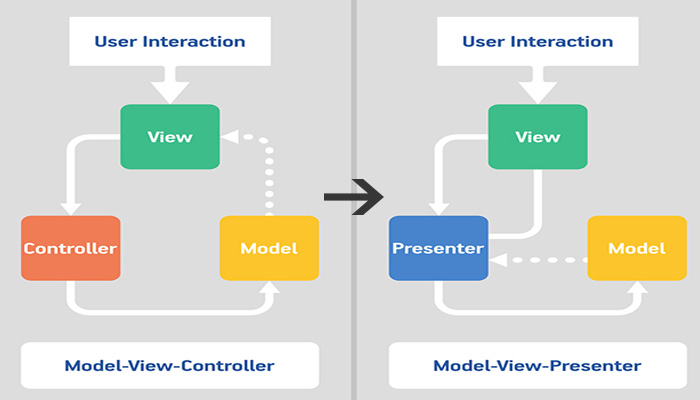
\includegraphics[width=0.65\textwidth]{immagini/mvc-vs-mvp.jpg}
     \caption{MVC vs MVP.}\label{fig:MVC vs MVP}
   \end{figure}

   \newpage


   \subsection{Model}
   Il Model \'e un'interfaccia dedicata all'acceso dei dati di un'applicazione, si occupa quindi di fornire un'astrazione del modello dei dati presenti nel database.\\
   Il Model oltre a contenere la struttura dei dati da visualizzare si occupa anche di fornire una buona astrazione dei dati presenti nel database, modificando, aggiungendo e separando alcuni dei dati, in modo da rendere l'accesso e la visualizzazione dei dati pi\'u semplice per gli altri due componenti del pattern (View, Presenter).\\
   Un esempio potrebbe essere il seguente:
   Il database contiene una tabella con due tipi di dato:

   \begin{enumerate}
   \item \textbf{Nome}: String
   \item \textbf{DataDiNascita}: Date
   \end{enumerate}

   Quando il programma ricever\'a i dati dal database in un qualsiasi formato( Map, Json, Array..) il Model selezionerà i dati in base alla definizione data dal programmatore trasformando il risultato del database in un oggetto.
   Questo oggetto oltre a conserare le due informazioni ricevute dal database (Nome, DataDiNascita) potr'\a contenere ance informazioni aggiuntive inserite dal Model per facilitare l'uso e la manipolazione degli altri due componeti.
   In questo caso il modello potrebbe creare il nuovo campo "et\'a" facendo una semplice sottrazione fra due date, quella attuale e la data di nascita dell'utente.

   \begin{enumerate}
   \item \textbf{Nome}: String
   \item \textbf{DataDiNascita}: Date
   \item \textbf{Et\'a}: Int
   \end{enumerate}

   %https://medium.com/@cervonefrancesco/model-view-presenter-android-guidelines-94970b430ddf

   \subsection{View}
   La View \'e un' interfaccia che definisce cosa deve implementare il Presenter, affinch\'e possa interagire con l'interfaccia utente.\\
   La View interagisce con il Presenter per visualizzare i dati e notifica al Presenter le azioni che compie l'utente nell'interfaccia.\\
   La View pu\'o essere implementata da un Activity, un Fragment, o un widget Android, che contengono ProgressBar, TextView, RecyclerView o altri elementi che necessitano di essere aggiornarnati in base a qualche azione dell'utente o cambiamento nel server.\\
   Gli aggiornamenti della View possono essere gestiti in due diversi modi:
   \begin{itemize}
       \item Passive View
       \item Supervising Controller
   \end{itemize}

   Nella Passive View, il Presenter aggiorna la vista per applicare i cambiamenti del modello, in questa modalit\'a l'interazione con il Model è gestita esclusivamente dal Presenter, la vista quindi ha un comportamento "passivo" e non è a conoscenza dei cambiamenti nel Model.\\
   Ad esempio, se si dispone di un modulo username/password e di un pulsante "Invia", non si scrive la logica di validazione all' interno della View ma all' interno del Presenter. La View infatti dovrebbe solo contenere il nome utente e la password e inviarli al Presenter.

   Nel Supervising Controller, la vista interagisce direttamente con il Model per eseguire semplici operazioni di binding dei dati, senza l' intervento del Presenter. Il Presenter aggiorna il Model, e gestissce cambiamenti sulla View solo nei casi pi\'u complessi, ad esempio l'aggiurnameto di un colore in base alle modifiche effettuate su un dato del Model, poich\'e la modifica non prevede una corrispondenza diretta tra la View e il Model
   Entrambe le modalit\'a facilitano il testing delle view in Android poich\'e le loro implementazioni riducono al minimo la quantità di logica implementata nella View.

   \begin{figure}[!hb]
     \centering
     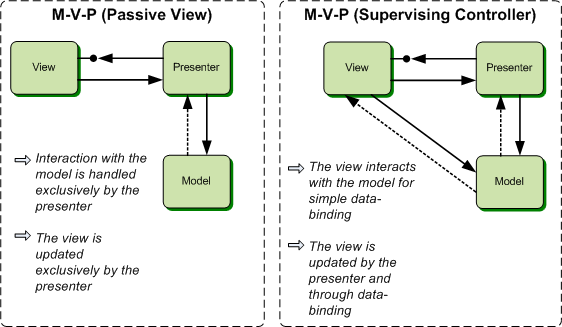
\includegraphics[width=0.7\textwidth]{immagini/mvp_view_types.png}
     \caption{MVP View types}\label{fig:Model View Types}
   \end{figure}

   \subsection{Presenter}
   Il Presenter \'e il mediatore tra il Model e la View e si occupa di  recuperare i dati dal Model, formattarli e passarli alla View, ma a differenza del pattern MVC, decide anche cosa succede quando si interagisce con la View reagendo alle interazioni dell'utente.\\
   Il Presenter per facilitare il testing deve cercare di non dipendere minimamente da Android, ma contenere solo metodi e dipendente Java, senza l'utilizzo del "Context" ad esempio, questo permetter\'a di scrivere i test per il Presenter senza l'utilizzo di un emulatore Android.\\
   Come detto in precedenza  il Presenter deve dipendere dall' interfaccia View e non direttamente dall' Activity o Fragment, in questo modo si tengono separati il Presenter e l'Activity rispettando la D dei principi SOLID:"Dipendi dalle astensioni. Non dipendere dalle concrezioni"\\










%%%%%%%%%%%%%%%%%%%%%%%%%%%%%%%%%%%%%%%%%non numera l'ultima pagina sinistra
\clearpage{\pagestyle{empty}\cleardoublepage}
